\documentclass[a4paper]{article}

\usepackage{amsmath}
\usepackage{amssymb}
\usepackage{parskip}
\usepackage{fullpage}
\usepackage{hyperref}
\usepackage{stellar}
\usepackage{chemfig}

\hypersetup{
    colorlinks=true,
    linkcolor=black,
    urlcolor=blue,
    pdftitle={Biology},
    pdfpagemode=FullScreen,
}

\newcommand{\quotes}[1]{``#1''}

\newcommand\hr{\par\vspace{-.5\ht\strutbox}\noindent\hrulefill\par\vspace{0.15cm}}

\title{Biology}
\author{Paolo Bettelini}
\date{}

\begin{document}

\maketitle
\tableofcontents
\pagebreak

% 978 88 6364 9437 (trovato)
% 978 88 6364 9635
% 978 88 6364 9659

\section{Sistemi}

\sdefinition{Sistema}{
    Un \textit{sistema} (vivente e non-vivente) è composto di parti differenti, specializzate e interdipendenti. 
    
    \begin{enumerate}
        \item Organizzazione della relazione fra le parti
        \item Struttura fisica, chimica etc. 
        \item Processo di riproduzione
    \end{enumerate}
}

\sdefinition{Emergenza Sistemica}{
    Una \textit{emergenza sistemica} è lo scopo che le diverse parti riescono ad raggiungere ed eseguire.
}

\sdefinition{Molecola organica}{
    Una molecola organica contiene il carbonio (tranne \(CO_2\)).
    % più o meno
}

\subsection{Sistemi viventi}

\sdefinition{ATP}{
    ATP è un composto organico che provvede energia alle cellule per le loro funzioni.
}

I seguenti processi sono eseguiti da tutti gli organismi viventi.

\textbf{Nutrizione:}
Tutti gli organismi viventi si nutrono con del \quotes{cibo}, ossia materia.
In generale, gli esseri viventi necessitano di \(C\), \(O\), \(H\), \(N\), \(S\) e \(P\).
L'unico nutrimento della pianta è \(CO_2\) (materia inorganica), mentre
i nutrimenti degli animali sono materia organica.

\sdefinition{Autotrofo}{
    Un organismo \textit{autotrofo} può svolgere la propria funzione di nutrizione,
    elaborando alimenti inorganici mediante assunzione d'energia dal mondo inorganico.
}

\sdefinition{Eterotrofo}{
    Un organismo \textit{eterotrofo}
    si nutre di sostanze organiche prodotte dagli organismi autotrofi.
}

\textbf{Respirazione:}

Tutti gli organismi viventi respirano
\[
    C_6H_{12}O_6 + O_2 \rightarrow CO_2 + H_2O
\]
In assenza di ossigeno (si usa la materia organica per produrre energia), e alcuni organismi \textit{fermentano}.
Nel caso degli umani i muscoli respirano, se non c'è \(O\) fermentano e producono acido lattico
che deve successivamente essere smaltito.

Le piante respirano mediante la fotosintesi
\[
    CO_2 + H_2O \rightarrow C_6H_{12}O_6 + O_2
\]

\textbf{Si riproduce e ha un ciclo vitale}

\textbf{Evolve}

\textbf{È sensibile (sa rispondere all'ambiente)}

\textbf{Mantiene stabili le sue condizioni interne}

\sdefinition{Biotico}{
    Con \textit{biotico} si intende tutto ciò che è vivente o era vivente.
} % foglia morta, elefante

\sdefinition{Abiotico}{
    Con \textit{abiotico} si intende tutto ciò che non è vivente e non lo è mai stato.
} % roccia

\sdefinition{Detrito}{
    Con \textit{detrito} si intende il resto di ogni organismo vivente che è morto.
} % foglia morta

Il sistema vivente presenta le medesima ma caratteristiche del sistema non-vivente,
ma possiede anche le seguenti componenti.

\sdefinition{Componente}{
    Insieme di materia, concreta e tangibile
}

\sexample{Components}{
    Acqua, suolo, sali minerali, ossigeno.
}

\sdefinition{Fattore}{
    Derive dalla presenza di componenti, produce un determinato effetto o risultato e si può misurare.
}

\sexample{Fattore}{
    \begin{itemize}
        \item Decomposizione (fattore biotico).
        \item Predazione, catena alimentare (fattore biotico).
        \item Vento (fattore abiotico).
        \item Luce solare (fattore abiotico).
        \item Luce della lucciola (fattore biotico).
    \end{itemize}
}

Un fattore rappresenta tutto ciò che si può misurare e che non è una componente.

\subsubsection{Autopoiesi}

\sdefinition{Autopoiesi}{
    La capacità di ripararsi, modificarsi e riprodursi da solo, internamente ed in maniera autonoma.
}
I sistemi viventi sono organizzativamente chiusi, per cui hanno un confine.

\sexample{Sistema autopoietico - ciclo}{
    TODO: mettere foto
}

\sexample{Sistema autopoietico - cellula}{
    TODO: mettere foto
}

\subsubsection{Dissipazione}

\sdefinition{Dissipazione}{
    La necessità di consumare energia, materia ed informazioni dall'esterno.
}
I sistemi viventi sono metabolicamente aperti, per cui hanno degli scambi con l'esterno
e rinnovano il proprio materiale.

\subsubsection{Cognizione}

\sdefinition{Cognizione}{
    L'attiva conoscenza dell'ambiente, esterno ed interno, da parte del sistema.
}

\section{Biomolecole}

\sdefinition{Biomolecola}{
    Le \textit{biomolecole} sono le molecole dei processi biologici degli essere viventi.
}

Tutte le biomolecole contengono \(C\), \(O\) e \(H\).
Ci sono delle eccezioni, per esempio, gli idrocarburi contengono solamente \(C\) e \(O\).

Le biomolecole sono di 4 tipi:
\begin{itemize}
    \item Lipidi (grasso)
    \item Acidi nucleici (DNA e RNA)
    \item Carboidrati
    \item Proteine
\end{itemize}

Le macromolecole sono composte da \textit{monomeri} e \textit{polimeri}.
Nel corpo umano i polimeri sono creati dalle cellule mediante alle istruzioni nel DNA.
Le biomolecole fanno dei polimeri.

\sdefinition{Isomero}{
    Gli \textit{isomeri} sono delle molecole distinte con il medesimo numero di atomi,
    ma con una struttura diversa. Diversi isomeri potrebbero avere proprietà diverse.
}

\paragraph{Costruzione di polimeri}

Tutti i monomeri posseggono, da una parte un gruppo di idrogeno \(H\),
e dall'altra un gruppo \(OH\).
Due monomeri si uniscono mediante una reazione chimica chiamata \textit{condensazioe} o \textit{disidratazione}, la quale consiste
nell'unire un'estremità \(H\) con una \(OH\) mediante un legame.
La condensazione libera una molecola d'acqua come scarto.

\paragraph{Disintegrazione di polimeri}

Per separare un legame fra due monomeri, viene utilizzata la reazione chimica di \textit{idrolisi} o \textit{idratazione}.
Questa reazione necessita di una molecola di \(H_2O\).

\pagebreak

\subsection{Carboidrati}

\sdefinition{Carboidrato}{
    I \textit{carboidrati} sono dei tipi di biomolecole composti da carbonio, idrogeno e ossigeno
    \((CH_2O)_n\).
}

I monomeri di carboidrati si chiamano monosaccaridi.
I polimeri di carboidrati si chiamano polisaccaridi (disaccaridi, trisaccaridi)

\sdefinition{Maltosio}{
    Il \textit{maltosio} è composto da due molecole di glucosio (\(C_{12}H_{22}O_{11}\)).
}

Per unire 2 molecole di glucosio
è necessario perderne una di \(H_2O\). Per cui il maltosio è dato da \(C_{12}H_{22}O_{11}\).

\sdefinition{Saccarosio}{
    Il \textit{saccarosio} è composto da un glucosio e un fruttosio (\(C_{12}H_{22}O_{11}\)).
}
\sdefinition{Lattosio}{
    Il \textit{lattosio} è composto da un glucosio e un galattosio (\(C_{12}H_{22}O_{11}\)).
}

I monosaccaridi sono glucosio, fruttosio, galattosio (isomeri).

\sdefinition{Amido}{
    L'\textit{amido} è un polisaccaride che viene prodotto dalle piante.
    Esso è composto da una catena di glucosi arrotolati ad elica.
}

L'\textit{amilasi} è l'enzima che rompe l'amido.
Esso fa parte della famiglia degli \textit{idrolasi}, ossia tutti gli enzimi che
eseguono l'idrolisi.

\sdefinition{Glicogeno}{
    Il \textit{glicogeno} è un polisaccaride che viene prodotto dagli animali.
    Esso è composto da diverse diramazioni di catene di glucosio.
}

Amido e glicogeno occupano meno spazio dei monomeri da soli, per cui sono ottimali per immagazzinare
il glucosio.

Gli esseri umani immagazzinano il glucosio in eccesso nei muscoli e nel fegato, dove ci sono degli enzimi
che sono in grado di creare questi polimeri di glucosio.

\sdefinition{Cellulosa}{
    La \textit{cellulosa} è un polisaccaride di glucosio prodotto dalle piante.
    Esso è composto un insieme di fibre lineari.
}

La cellulosa serve per dare rigidità al tessuto delle piante.

I polisaccaridi sono amido, glicogeno e cellulosa.

% Sintesi dello sciroppo di mais

\pagebreak

\subsection{Proteine}

I monomero di proteine si chiamano \textit{amminoacidi}.

% TODO foto

Ci sono 20 possibili amminoacidi diversi.

\sdefinition{Catena Polipeptidica}{
    Una \textit{catena polipeptidica} è una catena di amminoacidi.
}

\sdefinition{Proteina}{
    Le \textit{proteine} sono delle biomolecole costruite
    da una o più catene polipeptidiche.
}

Le proteine si distinguono in 7 classi per funzione
\begin{enumerate}
    \item \textbf{Strutturali:} es. unghie (cheratina).
    % Elastina, Collagene

    \item \textbf{Contrattili:} costituiscono il muscolo.
    % Actina e Miosina

    \item Di \textbf{riserva:} costituiscono una riserva di amminoacidi (specialmente per l'embrione).
    % Es. Albumina, Caseina

    \item Di \textbf{difesa:} costituiscono gli anticorpi, neutralizzano gli agenti patogeni.
    
    \item Di \textbf{trasporto:} trasportano l'ossigeno all'interno del sistema circolatorio.
    % Emoglobina

    \item \textbf{Regolatrici:} costituiscono alcuni ormoni.
    % Insulina

    \item \textbf{Enzimi:} costituiscono gli enzimi.
\end{enumerate}

\pagebreak

\subsection{Lipidi}

\sdefinition{Lipido}{
    I \textit{lipidi} sono un insieme di molecole idrofobe.
}

I lipidi non sono strutturati con monomeri e polimeri.

I lipidi vengono categorizzati nelle seguenti classi:

\subsubsection{Trigliceride}

\sdefinition{Trigliceride}{
    Il \textit{trigliceride} è una riserva energetica della cellula (comunemente grasso).
}

Il monogliceride è composto da un glicerolo, attaccato (per condensazione) ad un acido grasso.
Il trigliceride è attaccato a 3 catene di acido grasso.

Le catene di acidi grassi possono essere dritti (saturi) oppure piegate (insaturi).
Alle catene insature mancano alcuni doppi legami.

\subsubsection{Fosfolipide}

\sdefinition{Fosfolipide}{
    Il \textit{fosfolipide} sono composti da una testa idrofila e da una code idrofoba.
}

Le catarriteristiche idrofobe e idrofile permettono ai fosfolipidi di disporsi in maniera ordinata,
con la testa verso l'acqua e la coda rivolta verso l'esterno.

\subsubsection{Steroidi}

\sdefinition{Steroide}{
    Lo \textit{steroide} è una molecola con una struttura di 4 anelli.
}

Alcuni esempi sono il colesterolo, testosterone ed estrogeno.

\pagebreak

\subsection{Acidi nucleici}

I monomeri degli aicid nucleici si chiamano \textit{nucleotidi}.
% polimero = acido nucleico
\sdefinition{Acido nucleico}{
    L'\textit{acido nucleico} è composto da un gruppo fosfato, zucchero e base azotata.
}

\sdefinition{DNA}{
    Il \textit{DNA} è composto da due filamenti di nucleotidi.
}

I nucleotidi del DNA sono 4 (A, C, G, T).

\pagebreak

\section{Bioenergetica}

\subsection{Le membrane}

\sdefinition{Membrana}{
    Le membrane sono dei fosfolipidi con una code e una testa idrofila.
}

Questi fosfolipidi si attraggono per polarità e possono formare le seguenti composizioni

\begin{figure}[h]
    \centering
    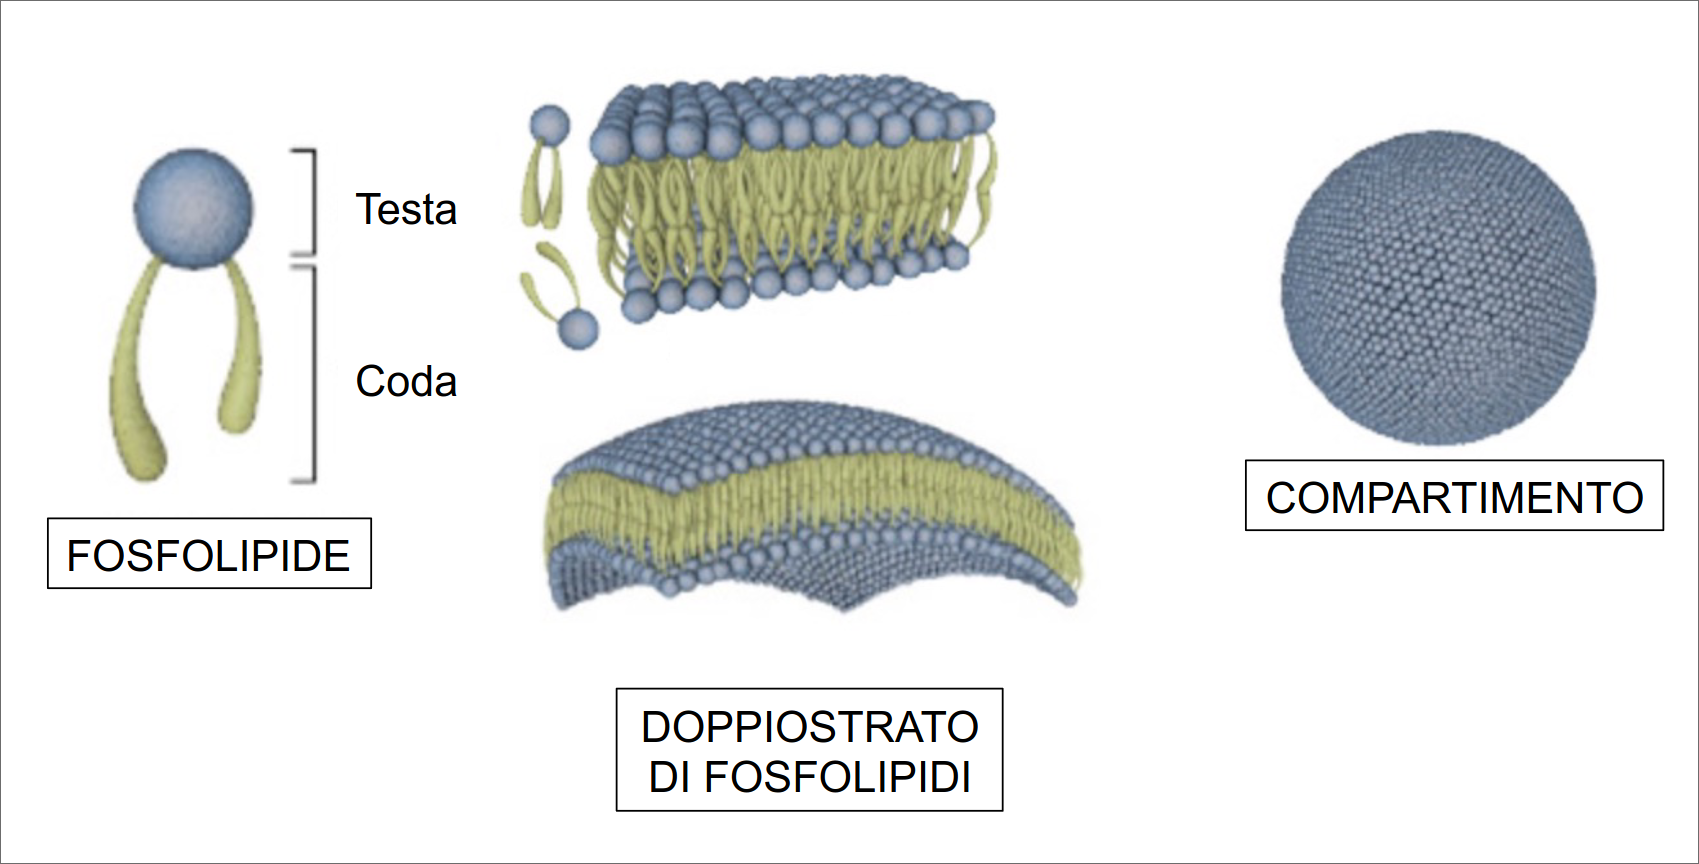
\includegraphics[width=\textwidth]{./membrana.png}
\end{figure}

Le sostanze idrofile (steroidi, grassi, etc.) vengono trasportati nel sangue

\subsubsection{Proteine di membrana}

\sdefinition{Gradiente di concentrazione}{
    Il \textit{gradiente di concentrazione} è un regolare incremento o diminuzione della concentrazione di una sostanza. Quando è presente un gradiente di concentrazione, gli ioni o le altre sostanze coinvolte tendono a muoversi spontaneamente dalla zona di concentrazione maggiore a quella di concentrazione minore.
}

Le principali tipologie di proteine che vengono incastrate nelle membrane sono:
\sdefinition{Proteina di trasporto}{
    Una \textit{proteina di trasporto} (canale) è una proteine di membrana che forma un tunnel sempre aperto.
}
Ogni canale non è direzionale ed ogni canale è specifico per un certo soluto.

\begin{figure}[h!]
    \centering
    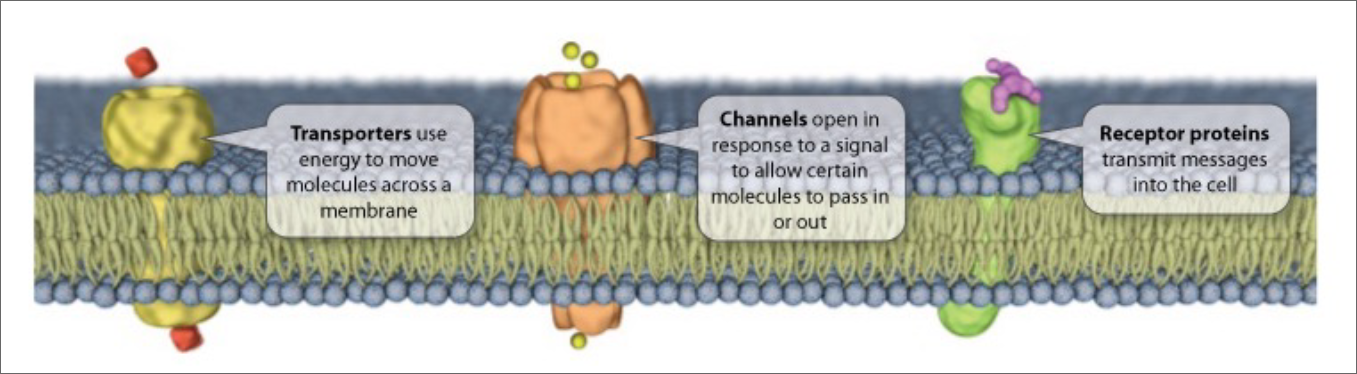
\includegraphics[width=\textwidth]{./proteine_mem.png}
\end{figure}

Tuttavia, siccome le cellule necessitano un ambiente interno diverso da quello esterno,
devono andare contro il gradiente di concentrazione.
Per risolvere questo problema vengono utilizzati i trasportatori.

\sdefinition{Trasportatore}{
    Un \textit{trasportatore} è una proteina che sposta una sostanza contro il gradiente.
}
Ogni tipo di trasportatore è specifico ad un tipo di sostanza.
Il trasportatore sposta quindi una sostanza da dove ce n'è poca a dove ce n'è tanta (mediante energia).

\sdefinition{Ricettori}{
    Un \textit{ricettore} è una proteina che comunica dei messaggi alla cellula.
}

\sexample{Ricettori}{
    Un ricettore potrebbe per esempio comunicare il segnale della presenza di un agente patogeno.
}

% todo fare 2 definitions
Alcune molecole possono passare direttamente attraverso la membrana, come per esempio l'azoto, l'ossigeno, acqua e glicerolo.
Questo movimento è detto diffusione semplice nei fosfolipidi. Chiaramente, la cellula non può controllare queste sostanze.

Le molecole grandi e ioni non passano per i fosfolipidi senza un canale (diffusione facilitata).

% grandiente elttrochimico con polarità

\sdefinition{Trasporto attivo primario}{
    Il trasporto attivo primario è un trasporto grazie ad un trasportatore e all'ATP.
}

Se non viene utilizzata direttamente l'ATP,
bensì viene sfruttata la differenza di gradiente di concentrazione stabilita da un trasporto primario,
si parla di trasporto \textit{secondario}.

% TODO secondario /? uniporto simporto antiproto

% TODO osmosi

\end{document}